\RequirePackage[T1]{fontenc}
\documentclass[conference,a4paper]{IEEEtran}
\usepackage{graphicx}
\usepackage{cite}
\usepackage{array}
\usepackage{url}
\usepackage[hidelinks]{hyperref}
\renewcommand{\dbltopfraction}{0.9}
\setcounter{dbltopnumber}{2}
\hyphenation{in-ter-oper-abil-ity tech-no-log-i-cal}
\begin{document}
\title{
\includegraphics[width=2.8cm]{assets/ulo_estg_logo.png}\\[6pt]
AeroEye}
\author{\IEEEauthorblockN{Daniel Santana, Gabriel Bernardes, Rúben Alves}
\IEEEauthorblockA{School of Technology and Management, University of Leiria and Oeste, Leiria, Portugal\\
2231161@ulo.pt, 2231170@ulo.pt, 2231034@ulo.pt\\
Emerging and Intelligent Technologies \textperiodcentered{} Virtual and Augmented Reality \textperiodcentered{} 2026/2027}}
\maketitle
\begin{abstract}
Replace this paragraph with a 150--200-word abstract stating the problem, review scope, literature selection, main findings and implications for the proposed project. Distinguish conclusions supported by the literature from benefits that still need validation. Do not report results for an unimplemented system. Replace all guidance, sample entries and author details before submission. The final paper must contain 6--8 pages including references.
\end{abstract}
\begin{IEEEkeywords}
state of the art; emerging technologies; virtual reality; augmented reality; project proposal
\end{IEEEkeywords}
\section{Introduction}
Introduce the application domain, intended users and problem. Explain its relevance and what existing approaches do not adequately address. Define the review objectives and scope, and explain how the review supports the multidisciplinary project topic approved by the lecturers. Include only the background needed to understand subsequent comparisons and decisions.

Explain how Emerging and Intelligent Technologies (EIT) and Virtual and Augmented Reality (VAR) contribute to the common problem. Justify the use of VR and/or AR for the intended task, considering a conventional alternative where relevant. Define essential terminology and abbreviations.

\subsection{Scope and literature search}
Identify where and when you searched, the main search terms and the criteria used to select material. State practical boundaries such as domain, device type or publication period. A short paragraph is sufficient; formal research questions, a systematic review protocol and a PRISMA diagram are not required. Acknowledge limitations.

\section{State of the Art}
A integração de Veículos Aéreos Não Tripulados (UAVs) e sistemas autónomos tem vindo a intensificar-se com a transição da Indústria 4.0 para a Indústria 5.0, onde a colaboração homem-máquina e a automação sustentável assumem um papel central. Esta evolução tem impulsionado investigações relevantes focadas na aplicação de robótica aérea em ambientes operacionais complexos. Como tal, a presente secção dedica-se a contextualizar o estado da arte e a literatura científica existente em torno desta temática.

%sensores usados, ambientes indoor/outdoor, como a VR é usada nas diferentes abordagens, como a AR é usada

\subsection{Evolução Bibliométrica e Crescimento do Interesse Científico}
O estudo, desenvolvimento e implementação de drones em ambientes fabris e industriais registaram um crescimento notável nos últimos anos. De acordo com o levantamento bibliométrico conduzido por Mourtzis et al. \cite{Mourtzis02052024}, realizado em novembro de 2022 nas bases de dados \textit{Scopus}, \textit{Google Scholar} e \textit{Web of Science}, foram identificados 329 artigos científicos dedicados à temática. Uma análise de coocorrência de termos com recurso ao software \textit{VOSviewer} revelou que expressões como \textit{drones}, \textit{path planning} e \textit{antennas} figuram entre os principais focos de investigação.

Mais recentemente, uma consulta preliminar no \textit{Google Scholar}, utilizando o mesmo criterio de pesquisa, passou a retornar mais de 800 publicações indexadas, evidenciando uma tendência contínua de expansão da comunidade científica neste domínio e a premência de novas abordagens operacionais e algorítmicas.

\subsection{Domínios de Aplicação dos UAVs}
Atualmente, no contexto industrial, os veículos aéreos não tripulados (UAVs) podem ser empregados numa vasta gama de aplicações, incluindo a gestão de inventários, a otimização de armazéns e a logística de expedição e distribuição. Por exemplo, os UAVs são utilizados no reconhecimento aéreo de infraestruturas fabris para monitorizar níveis de stock, identificar potenciais estrangulamentos no processo produtivo e rastrear a movimentação de mercadorias ao longo da cadeia de abastecimento. Adicionalmente, estes sistemas viabilizam o transporte e a entrega autónoma de bens, reduzindo a necessidade de intervenção humana direta e aumentando a eficiência operacional global \cite{Mourtzis02052024}.

Para além do ambiente estritamente industrial, a literatura reporta a integração bem sucedida de UAVs numa ampla variedade de setores estratégicos, destacando-se:
\begin{itemize}
    \item \textbf{Setor Energético:} Inspeção de proximidade em infraestruturas e linhas de transporte elétrico através de câmaras térmicas e de alta resolução, permitindo detetar falhas operacionais e danos estruturais de forma mais rápida e segura do que os métodos convencionais \cite{8801830}.
    \item \textbf{Agricultura de Precisão:} Monitorização aérea com recurso a sensores multiespectrais para análise e mapeamento dos níveis de azoto na vegetação, otimizando a aplicação direcionada de fertilizantes e aumentando o rendimento das culturas \cite{agronomy12091992}. %o "de precisao" secalhar vai com o crl
    \item \textbf{Construção Civil:} Levantamentos topográficos e mapeamento 3D de estaleiros de obras, facilitando o pré-planeamento logístico, a gestão de riscos e a alocação eficiente de recursos \cite{rs12142329}.
    \item \textbf{Indústria Extrativa e Mineração:} Uso de tecnologia \textit{Light Detection and Ranging} (LiDAR) para gerar modelos topográficos de elevada fidelidade, viabilizando a deteção preventiva de zonas de instabilidade geológica e perigo de desabamento rochoso \cite{rs18091333}.
    \item \textbf{Saúde:} Utilização de drones para monitorizar indicadores de saúde de pessoas com suspeita de infeção por COVID-19, nomeadamente através da medição da temperatura corporal e da análise da respiração.
    \item \textbf{Guerra:} Usado para detetar inimigos e armadilhas, assim como ambientes com materiais tóxicos e prejudiciais ao ser humano
    \item \textbf{Desastres:} Utilizado para localizar escombros e possiveis locais com sobreviventes.\cite{jsan14050098}
\end{itemize}

%posso adicionar o uso em conflitos armados, desastres e ???ambientes perigosos??? , saude (COVID)... (FEITO) tenho citation... Mas estar a espetar todos os exemplos em lista nao sei se é assim que o prof quer...

Os exemplos apresentados evidenciam a versatilidade dos UAVs para efetuar o levantamento de dados em cenários operacionais distintos. Apesar da diferença significativa em relação ao objetivo de cada projeto apresentado, verifica-se uma abordagem transversal: a recolha de dados importantes através de sensores e a sua posterior disponibilização em dashboards ou outras interfaces de visualização, com o propósito de auxiliar o processo de tomada de decisão.

% merdas a falar
% uso de AR para aasistencia na monutenção de X
% controlo/ver de drones via VR
% servidor centralizado com as informações recolhidas
\subsection{IoT e aquisiçao de dados em ambientes industriais}

A Internet of Things (IoT) permite interligar dispositivos físicos através de redes de comunicação, possibilitando a troca de informação entre estes e a Internet. Estes dispositivos recorrem frequentemente a sensores para recolher dados do meio envolvente, permitindo a sua análise e a adaptação do comportamento dos sistemas em função do contexto.

A adoção crescente desta tecnologia tem registado um crescimento de tal forma elevado nos últimos anos, que se estima que o número de \textit{smart devices}, que se situava nos 21 mil milhões no final de 2025, venha a mais do que duplicar, atingindo os 48 mil milhões até 2035 \cite{transforma2026iot}.

No contexto industrial, a IoT assume a designação Industrial Internet of Things (IIoT), correspondente à aplicação desta tecnologia no âmbito industrial, nomeadamente em equipamentos e processos industriais. A recolha contínua de dados permite acompanhar o estado dos equipamentos, identificar alterações nas suas condições de funcionamento e disponibilizar informação relevante para a análise e o diagnóstico de possíveis anomalias.


A recolha de dados através de sensores constitui apenas uma das componentes de um sistema de monitorização industrial. Para que a informação recolhida seja útil aos operadores, é necessário disponibilizá-la de forma organizada e compreensível, permitindo acompanhar o estado dos equipamentos e analisar a evolução dos parâmetros monitorizados.

Neste contexto, os dashboards constituem uma das principais formas de visualização da informação operacional, recorrendo a indicadores, gráficos, históricos e alertas para facilitar a interpretação dos dados. Contudo, a eficácia destas interfaces não depende apenas da quantidade de informação apresentada, mas também da forma como esta é organizada e relacionada com o contexto operacional. Estudos sobre interfaces de monitorização industrial demonstram que diferentes formas de apresentar a mesma informação podem influenciar a compreensão da situação pelos operadores \cite{doi:10.1177/154193121005400411}.

A integração de sensores, sistemas de processamento de dados e interfaces de visualização permite, assim, desenvolver soluções de monitorização que facilitam o acompanhamento dos equipamentos e a identificação de comportamentos que justifiquem uma análise mais aprofundada \cite{reis2024infraestrutura}. Esta informação pode também servir de suporte ao diagnóstico de anomalias, constituindo uma base para soluções de assistência remota que disponibilizem aos operadores e técnicos o contexto necessário para avaliar as situações identificadas.

\subsection{Realidade Virtual e Aumentada na monitorização industrial}
\subsection{Integração de IoT com VR e AR}
\subsection{Servidor central}


% -------------------- Template --------------------
\subsection{template}

Organise the literature by approaches, themes or comparison criteria. Compare what the studies attempted, the contexts in which they were evaluated, the evidence they produced and the limitations reported. Avoid a sequence of unrelated summaries. Distinguish measured results from authors' expectations, and explain when differences in tasks, datasets, participants or hardware prevent direct comparison.

Use scientific studies for evidence about performance and evaluation, and official documentation for tool capabilities. Foundational literature, such as Azuma's survey \cite{azuma1997}, may provide context; complement it with recent studies relevant to your problem. This example reference does not replace the group's literature selection. IEEE provides the original formatting guidance \cite{ieeeauthor}.

\subsection{Comparative synthesis}
Table~\ref{tab:comparison} illustrates a comparison matrix spanning both columns. Its entries are hypothetical prompts, not published findings. Replace them with evidence from the studies you actually analysed, identifying each source. Select criteria that support a decision in your project. In the text, explain the main patterns, disagreements and gaps revealed by the table; a table alone is not a critical synthesis.

\begin{table*}[!t]
\caption{Illustrative literature comparison matrix spanning both columns}
\label{tab:comparison}
\centering
\footnotesize
\setlength{\tabcolsep}{4pt}
\renewcommand{\arraystretch}{1.18}
\begin{tabular}{|>{\raggedright\arraybackslash}p{0.13\textwidth}|>{\raggedright\arraybackslash}p{0.19\textwidth}|>{\raggedright\arraybackslash}p{0.21\textwidth}|>{\raggedright\arraybackslash}p{0.18\textwidth}|>{\raggedright\arraybackslash}p{0.19\textwidth}|}
\hline
\textbf{Study / source} & \textbf{Context and approach} & \textbf{Evidence to extract} & \textbf{Limitation to check} & \textbf{Decision informed} \\ \hline
Study A (replace) & AR task guidance & Task time, errors, sample and protocol & Task specificity; device constraints & Interaction and comparison baseline \\ \hline
Study B (replace) & VR training simulation & Performance, usability and transfer measures & Transfer to real tasks; exposure time & Training scenario and validation plan \\ \hline
Study C (replace) & Sensor-backed service & Latency, reliability and test conditions & Network dependence; controlled setting & Processing location and interface design \\ \hline
\end{tabular}
\vspace{3pt}
\parbox{\textwidth}{\footnotesize The rows above are illustrative prompts, not results from real studies. Replace them with analysed sources and verified evidence.}
\end{table*}

\section{Technological Analysis}
O desenvolvimento do sistema AeroEye exige a integração de múltiplos módulos de software, desde a deteção de anomalias até às interfaces imersivas e serviços web. De forma a garantir escolhas fundamentadas, as linguagens de programação, \textit{frameworks} e motores considerados foram avaliados com base em critérios explícitos: latência de execução, restrições de recursos computacionais, maturidade do ecossistema e esforço de desenvolvimento no espaço temporal de um semestre letivo. Esta secção justifica as opções adotadas e analisa as principais alternativas tecnológicas.

\subsection{Deteção de Anomalias e Visão computacional}
A inspeção autónoma de maquinaria assenta em algoritmos de visão computacional e \textit{machine learning}. As opções ponderadas foram C++ e Python. Embora C++ ofereça menor latência e reduzido \textit{overhead} de memória em sistemas embebidos, optou-se por Python devido ao seu ecossistema robusto de bibliotecas de aprendizagem automática. Esta escolha otimiza o esforço de desenvolvimento e a velocidade de prototipagem dentro do prazo estipulado.

\subsection{Ambiente de Realidade Virtual (VR)}
A interface de diagnóstico remoto requer uma aplicação de Realidade Virtual (VR) capaz de receber o \textit{stream} de vídeo em tempo real e permitir o controlo do drone. Avaliaram-se o WebXR, o Unreal Engine e o Unity. O WebXR, apesar de prescindir de um motor de jogo, apresenta elevada complexidade de implementação. O Unreal Engine oferece elevado rigor gráfico, mas consome mais recursos e exige desenvolvimento em C++. Assim, selecionou-se o Unity pela flexibilidade do C\#, menor consumo de recursos e compatibilidade imediata com diversos \textit{headsets} VR.

\subsection{Interface de Realidade Aumentada (AR)}
Para apoiar os operadores no terreno através de notas contextuais sobre os equipamentos, definiu-se uma aplicação móvel para Android. Descartou-se o WebAR devido a limitações de desempenho e acesso restrito ao \textit{hardware}. A utilização do Unity AR Foundation também foi ponderada, contudo, manter o motor Unity em segundo plano gera um consumo computacional e de bateria desnecessário. Por conseguinte, escolheu-se o desenvolvimento nativo em Kotlin com ARCore, assegurando acesso direto aos sensores e à câmara do dispositivo com reduzido impacto no sistema.

\subsection{Servidor Central e Camada de API}
A persistência de dados, a gestão da telemetria do drone e a comunicação entre módulos exigem um serviço central robusto. Selecionou-se o Laravel (PHP) para a construção da API RESTful e Laravel Reverb para \textit{WebSockets}. Em comparação com \textit{frameworks} minimalistas em Node.js ou Python, o Laravel oferece uma arquitetura MVC consolidada com mecanismos nativos de autenticação, ORM e estruturação de dados, acelerando o desenvolvimento e garantindo a segurança do sistema.

\subsection{Dashboard de Gestão}
Para apresentar os relatórios de inspeção, dados recolhidos pelo drone e estado das máquinas aos gestores industriais, desenvolve-se uma \textit{dashboard} web. Ponderaram-se as \textit{frameworks} React e Vue.js. A opção recaiu sobre o Vue.js, uma vez que a gestão de estado reativo através do Pinia simplifica a sincronização de dados em tempo real com a API central.

\section{Project Proposal}
\subsection{Solução e Arquitetura Conceitual}
A solução proposta destina-se a gestores e responsáveis de manutenção em ambiente industrial. A ideia consiste em utilizar um drone, que realiza rondas regulares pelo interior de uma fábrica e verifica o estado das máquinas. O objetivo principal é detetar anomalias o mais cedo possível, tirando partido da recolha de dados de múltiplos sensores (câmara, temperatura e ruído) e de uma interface imersiva dupla, combinando realidade virtual para o controlo remoto do drone e a realidade aumentada para o apoio técnico no terreno. O âmbito do sistema foca-se exclusivamente na monitorização e diagnóstico de anomalias no interior das instalações, deixando de fora qualquer tipo de reparação física. \\

No âmbito da unidade curricular Tecnologias Emergentes e Inteligentes, o sistema foca-se na recolha e transmissão contínua de dados dos sensores presentes no drone, enviando os mesmos para um servidor central através de uma API, posteriormente seguindo para uma dashboard central que disponibiliza a lista de máquinas, o respetivo estado atual, as características técnicas, o histórico de avarias e estatísticas de anomalias na fábrica. \\

No que diz respeito à unidade curricular Realidade Virtual e Aumentada, a arquitetura integra duas vertentes complementares: um operador remoto pode pilotar o drone utilizando óculos de realidade virtual e registar anotações digitais sobre a resolução da anomalia em questão e, posteriormente, um técnico no terreno aproxima-se da máquina com um telemóvel com realidade aumentada, visualiza as instruções deixadas pelo especialista e executa a intervenção tendo em conta as mesmas. \\

Referente aos componentes principais, a solução é constituída pelo drone (equipado com sensores e um dispositivo de processamento complementar), pela dashboard central de monitorização, pelos óculos VR e pelo smartphone com suporte a AR, apoiados por um servidor. A comunicação e as interfaces de integração baseiam-se em protocolos de rede sem fios para a transmissão em tempo real, fluxo de vídeo e dados analíticos. O sistema incorpora um mecanismo de resiliência a falhas de rede, em que os dados são armazenados localmente no drone, para posterior sincronização assim que a conectividade for restabelecida. \\

Por fim, a Figura~\ref{fig:solution_architecture} ilustra o diagrama de arquitetura global da solução, evidenciando a integração direta entre a interface imersiva, os serviços de processamento e as respetivas fontes de dados. \\

\begin{figure*}[!t]
    \centering
    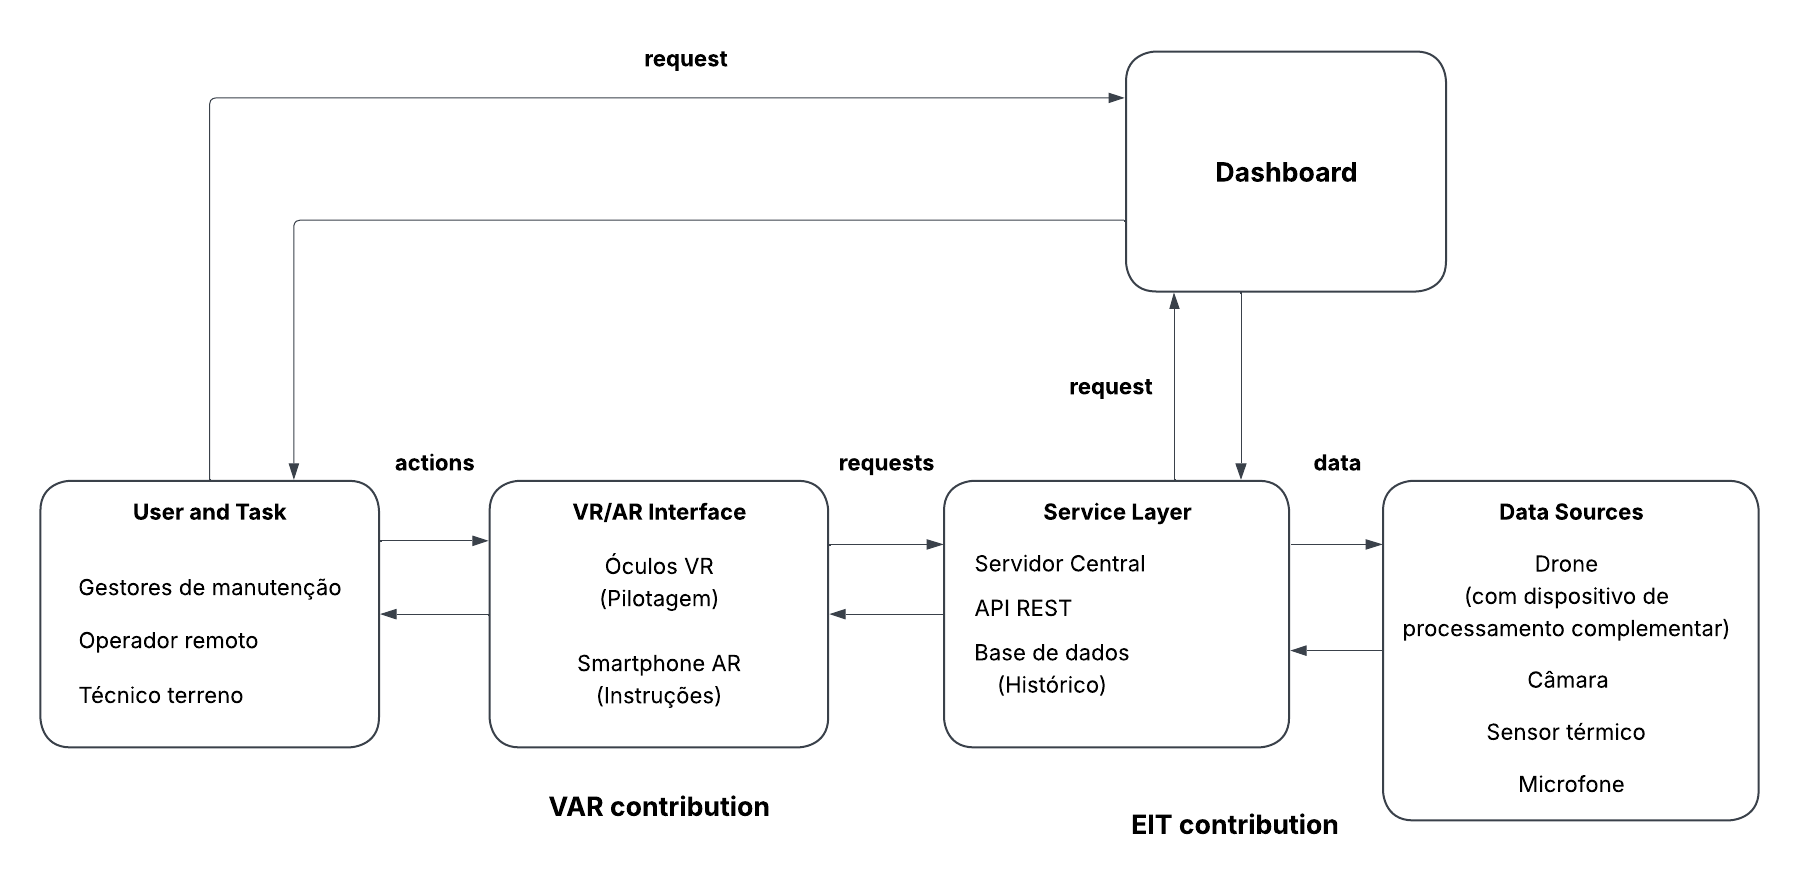
\includegraphics[width=\textwidth]{assets/Arquitetura EIT_RVA.png}
    \caption{Arquitetura conceptual da solução.}
    \label{fig:solution_architecture}
\end{figure*}

A Figura~\ref{fig:solution_architecture} apresenta a arquitetura da solução, integrando os utilizadores, as interfaces imersivas, a camada de serviços e as fontes de dados. O diagrama indica o caminho dos fluxos de informação entre cada bloco, os pontos onde o processamento é executado e a divisão entre as unidades curriculares de Tecnologias Emergentes e Inteligentes e Realidade Virtual e Aumentada.\\

\textbf{Fluxos de Dados e Níveis de processamento}
As setas bidirecionais demonstram a comunicação contínua entre os diferentes blocos:
\begin{itemize}
    \item \textbf{User and Task $\leftrightarrow$ VR/AR Interface / Dashboard:} O operador remoto realiza \textit{actions} (comandos de voo e interações) utilizando a interface VR, enquanto o técnico no terreno visualiza as instruções de apoio em AR. Paralelamente, os utilizadores enviam requests para a Dashboard para consultar informações.
    \item \textbf{Dashboard $\leftrightarrow$ Service Layer:} A \textit{Dashboard} realiza \textit{requests} ao servidor para obter e apresentar a informação.
    \item \textbf{VR/AR Interface $\leftrightarrow$ Service Layer:} As aplicações de VR e AR enviam pedidos constantes à API REST para carregar o vídeo e os dados em tempo real, respetivamente.
    \item \textbf{Service Layer $\leftrightarrow$ Data Sources:} O Servidor Central utiliza a API REST para enviar comandos ao dispositivo complementar do drone, enquanto este envia de volta o vídeo, os valores de temperatura e de ruído, que o servidor guarda na base de dados para atualizar o histórico.
\end{itemize}

\textbf{Dependências do Sistema}
\begin{itemize}
    \item \textbf{Equipamento:} Drone autónomo equipado com câmara, sensor térmico e microfone, óculos de Realidade Virtual, \textit{smartphones} compatíveis com AR e servidor central(API REST e base de dados para histórico).
    \item \textbf{Software:} Unity para a aplicação VR, Kotlin com ARCore para a interface AR e Laravel com Vue.js para gerir a API REST e a \textit{Dashboard}.
    \item \textbf{Dados e Serviços:} Utilização de \textit{WI-FI} 5 para comunicação entre o servidor central, o drone e os óculos VR e a aplicação AR. O servidor central encontra-se ligado por cabo Ethernet, sendo complementado por um serviço de base de dados para garantir a integridade do histórico. 
\end{itemize}

\textbf{Plano Preliminar de Desenvolvimento}
\begin{enumerate}
    \item \textbf{Requisitos e Arquitetura:} Desenho do esquema da base de dados, mapeamento de \textit{endpoints} da API e aquisição de equipamentos.
  % tipo em esoft de dizer, drone -> enconrtea anomalia -> envia para o server -> envia ao telemovel. Telemovel em modo controlo -> server -> drone -> cenas
    \item \textbf{Infraestrutura Central:} Desenvolvimento da \textit{Service Layer} (servidor e API REST) e implementação da \textit{Dashboard}.
    \item \textbf{Integração de Edge:} Configuração computacional no drone, calibração dos três sensores (câmara, térmico, microfone) e estabelecimento da comunicação com o servidor.
    \item \textbf{Prototipagem Imersiva:} Desenvolvimento e integração das aplicações clientes para os óculos VR (focada na pilotagem e anotação no ambiente) e para o \textit{smartphone} com AR (focada na visualização instruções técnicas).
    \item \textbf{Validação Global:} Testes de carga e latência num ambiente industrial simulado para aferir a robustez da comunicação em tempo real. Testes para validar a persistência dos dados no ambiente virtual para realidade aumentada, verificando se as anotações permanecem na mesma posição e rotação. Testes para verificar a taxa de falsos positivos e falsos negativos nas deteções das anomalias realizadas pelo modelo. Testar a fiabilidade da recolha de dados pelos sensores do drone, nomeadamente o microfone e o sensor de temperatura.Adicionalmente, avaliar a facilidade de utilização dos diferentes componentes tecnológicos do sistema, incluindo a aplicação móvel, destinada ao controlo e à visualização do drone, os óculos de realidade virtual, utilizados para autenticação, controlo, visualização e criação de anotações, e a dashboard, tendo em conta a facilidade de navegação e de interpretação dos dados apresentados. Testar a fiabilidade da recolha de dados pelos sensores do drone, nomeadamente o microfone e o sensor de temperatura.
\end{enumerate}

\textbf{Escolhas Tecnológicas Provisórias}
Nesta fase inicial do projeto, algumas tecnologias e componentes continuam em avaliação. Deste modo, o dispositivo móvel para Realidade Aumentada, o dispositivo complementar do drone, a marca dos sensores, a tecnologia específica para a base de dados e o local de alojamento (\textit{host}) do servidor central permanecem em aberto. A consolidação destas escolhas depende

\subsection{Preliminary validation}
Define two or three evaluation criteria or metrics suited to the project. For each, explain what will be assessed, the proposed test, the resources or participants required, and the intended success criterion or how it will be established. Include an appropriate baseline or alternative when useful. Possible choices include task completion time, task errors, usability, interaction accuracy or end-to-end latency; select only those relevant to your objectives.

At this stage, describe how the solution could be validated. An implemented prototype, a completed user study and experimental results are not required. Label expected benefits as hypotheses and identify provisional targets as such. Distinguish the evaluation reported by the reviewed studies from the evaluation planned for your own project.

\section{Discussion}
Discuss the feasibility of the proposal in light of the literature, available resources and semester constraints. Explain the expected technical challenges, integration risks and limitations of the evidence. Consider user comfort, accessibility, privacy or other concerns where they arise from the proposed use. Identify the expected contribution and the assumptions that still need to be tested.

Explain how the review strengthened or changed the proposal, which alternatives were rejected and when decisions might need revision. A justified application, adaptation, integration or evaluation of existing technologies can provide a contribution; distinguish it from unproven novelty.

\section{Conclusions}
Summarise the review findings, resulting decisions and expected contribution. Return to the initial objectives and identify the next development and validation steps. Do not introduce new evidence or claim results that have not been obtained.

\section*{AI Use Declaration}
Os autores utilizaram o Gemini 3.8 Flash, ChatGPT 5.6 Luna e Claude 5.5 com o propósito de reescrita e formalização estilística de pequenas secções do texto originalmente redigido pelos autores. Todos os outputs foram cuidadosamente revistos, editados sempre que necessário e verificados quanto à precisão técnica e das referências. Os autores mantêm a inteira responsabilidade pelo conteúdo do trabalho submetido.\\

\bibliographystyle{IEEEtran}
\bibliography{references}
\end{document}
